\documentclass[10pt,twocolumn]{article}
\usepackage[margin=1in]{geometry}
\usepackage{graphicx}
\usepackage{amsmath,amssymb}
\usepackage{booktabs}
\usepackage{hyperref}
\usepackage{natbib}
\usepackage{xcolor}
\usepackage{caption}
\usepackage{subcaption}
\usepackage{url}
\usepackage{microtype}
\usepackage{float}
\usepackage{multirow}
\usepackage{listings}
\usepackage{inconsolata}
\usepackage{tikz}
\usepackage{pgfplots}
\usepackage{pgfplotstable}
\usetikzlibrary{arrows.meta,positioning,shapes.geometric,fit,backgrounds,calc}
\pgfplotsset{compat=1.18}

\lstset{
  language=Python,
  basicstyle=\ttfamily\scriptsize,
  keywordstyle=\bfseries\color[rgb]{0.13,0.29,0.53},
  stringstyle=\color[rgb]{0.31,0.54,0.16},
  commentstyle=\itshape\color[rgb]{0.5,0.5,0.5},
  numbers=left,
  numberstyle=\tiny\color{gray},
  numbersep=5pt,
  frame=single,
  framesep=3pt,
  breaklines=true,
  showstringspaces=false,
  captionpos=b,
  aboveskip=8pt,
  belowskip=4pt,
}

\bibliographystyle{unsrtnat}

\title{MemLayer: A Universal Encrypted Memory Layer for\\Cross-Provider LLM Context Efficiency}
\author{Abhishek Shekhar\\
\url{https://github.com/Abhi183/ai-memory-layer}}
\date{}

\begin{document}
\maketitle

\begin{abstract}
Large language models are inherently stateless: every session begins without
memory of prior interactions, forcing applications to re-transmit complete
conversation histories at cost that grows quadratically with session length.
We present MemLayer, a provider-agnostic memory layer that intercepts prompts
from any AI terminal --- Claude Code, GPT-4, Gemini, and Ollama --- retrieves
semantically relevant memories via pgvector cosine similarity with composite
re-ranking, and injects only the essential context. On a 50-conversation
synthetic evaluation set, MemLayer reduces average token consumption from
15,000 to 1,024 tokens per query (93.2\% Token Compression Ratio), with
Precision@5 $= 0.84$ and a median retrieval latency of 24~ms --- less than
3\% of typical LLM generation time. An integrated economics engine tracks
provider-specific cost savings in real time: a team of ten developers pays
\$61/month on Claude Sonnet~4.5 instead of \$847, a 92.8\% reduction. Unlike
Mem0~\citep{chhikara2025mem0} and MemGPT~\citep{packer2023memgpt}, MemLayer
requires no cloud account, encrypts all memories per-user with AES-256-GCM,
and integrates natively with Claude Code via the Model Context Protocol. All
code is released at \url{https://github.com/Abhi183/ai-memory-layer}.
\end{abstract}

% =====================================================================
\section{Introduction}
\label{sec:intro}
% =====================================================================

\noindent
Every session starts from zero. This is not a design limitation of any
particular product --- it is the fundamental operational mode of transformer-based
language models, which process a fixed context window and produce a response
without any persistent state across calls. When a developer returns to a
coding session the next morning, they must either re-describe their entire
project context or prepend last session's transcript. Both strategies pay for
information that was already paid for.

The cost structure is quadratic, not linear. At turn $N$ in a session, the
accumulated transcript spans $N$ turns; to continue the session, all $N$ prior
turns must be re-sent. The total tokens billed across a session of $N$ turns
grows as $O(N^2)$ relative to the information content, which grows only
linearly. A concrete example: a developer using Claude Code for one week,
conducting 20 sessions of 30 turns each at 500 tokens per turn, submits
$20 \times \sum_{i=1}^{30} 500i \approx 4.65$~million tokens. The actual new
content introduced is $20 \times 30 \times 500 = 300{,}000$ tokens. The
remaining 4.35~million tokens --- 93.5\% of the bill --- are redundant history.

Three prior approaches address this statelessness problem, but each carries
significant limitations for practical deployment:
\begin{enumerate}
  \item \textbf{MemGPT}~\citep{packer2023memgpt} introduces a compelling
    OS-metaphor with hierarchical memory (core, recall, archival) and explicit
    context paging. However, it requires deploying a dedicated LLM operating
    system, is designed primarily around self-hosted models, and cannot wrap
    existing CLI tools without reimplementing the entire interface layer.
  \item \textbf{Mem0}~\citep{chhikara2025mem0} achieves 90\% token reduction
    through an extract-consolidate-retrieve pipeline with an optional graph
    memory variant. It is, however, cloud-dependent by design, provides no
    per-user encryption, and its pipeline is tightly coupled to the OpenAI
    embedding API, precluding fully offline deployments.
  \item \textbf{LangMem}~\citep{chase2024langmem} focuses on persistent memory
    within the LangGraph agent framework. Its tight runtime coupling makes it
    ill-suited for CLI-native or provider-agnostic deployments; wrapping an
    arbitrary terminal AI tool requires rebuilding the application inside
    LangGraph.
\end{enumerate}

This paper presents MemLayer, which addresses all three gaps through a
different design point: a lightweight, provider-agnostic middleware layer that
sits between any AI terminal and any LLM provider. We investigate three specific
research questions:
\begin{enumerate}
  \item What token compression ratio does semantic retrieval achieve versus
    full-context and no-memory baselines, and how does it depend on retrieval
    quality (Precision@5)?
  \item Does composite scoring (combining cosine similarity, recency, and
    importance) measurably outperform pure cosine similarity, and what weight
    configuration is optimal?
  \item What is the real-money economic impact of memory compression across
    providers, and how does it scale with team size and query volume?
\end{enumerate}

% =====================================================================
\section{Background}
\label{sec:background}
% =====================================================================

\subsection{Long-Context LLMs}

\noindent
Context window capacity has expanded from 4K tokens (GPT-3) to 1M tokens
(Gemini~1.5~Pro) within three years~\citep{vaswani2017attention}. This trend
does not render memory compression unnecessary: pricing for frontier models
scales with input token count, and attention complexity scales quadratically
with sequence length. At \$3 per million tokens, a 1M-token context costs \$3
per query. MemLayer reduces average effective context to 1,024 tokens, bringing
the same query to approximately \$0.003.

\subsection{MemGPT}

\noindent
MemGPT~\citep{packer2023memgpt} frames long-context management as an operating
system problem, with \emph{core memory} (the in-context working set),
\emph{recall memory} (searchable prior interactions), and \emph{archival memory}
(external document stores). The model itself controls memory operations through
function calls that page content in and out. This is architecturally elegant
but operationally demanding: it requires an LLM capable of faithfully executing
memory management function calls, and the overhead of each paging decision adds
latency to every query.

\subsection{Mem0}

\noindent
Mem0~\citep{chhikara2025mem0} demonstrates that an extract-then-retrieve
pipeline can reduce token usage by approximately 90\% while maintaining response
quality on the LOCOMO benchmark~\citep{maharana2024locomo}. Its graph memory
variant further improves cross-session recall by maintaining entity
relationships. The reported 91\% improvement in factual consistency over
baseline is compelling, but the dependency on cloud infrastructure and absence
of end-to-end encryption make Mem0 unsuitable for privacy-sensitive enterprise
or personal deployments.

\subsection{LangMem}

\noindent
LangMem~\citep{chase2024langmem} is designed as a native extension to the
LangGraph agent framework. It focuses on prompt refinement through memory:
accumulated facts are used to adapt system prompts for future sessions. While
effective within LangGraph applications, it does not provide a universal
adapter for arbitrary CLI-based LLM access patterns, and its architecture
requires opt-in at application build time rather than functioning as a
transparent wrapper.

\subsection{KV Cache Compression}

\noindent
KVzip~\citep{he2025kvzip} and related work compress key-value caches at the
hardware level to reduce memory bandwidth pressure during inference. This
approach is \emph{complementary} rather than competing: KV cache compression
operates within a single inference context window, while MemLayer operates at
the application layer to reduce what is sent in the first place. The two
can be combined.

\subsection{Retrieval-Augmented Generation}

\noindent
RAG~\citep{lewis2020retrieval} retrieves \emph{documents} relevant to a query
and injects them into context. MemLayer retrieves \emph{personal interaction
memories} --- extracted facts and summaries from prior sessions with a specific
user. The distinction matters for retrieval design: document chunks are
typically static, while personal memories have dynamic importance, age, and
relevance that must inform retrieval scoring. A-MEM~\citep{xu2025amem} explores
Zettelkasten-inspired memory notes for agents; MemLayer targets the simpler but
ubiquitous CLI use case and extends the design with provider-specific cost
accounting and per-user encryption.

% =====================================================================
\section{System Architecture}
\label{sec:architecture}
% =====================================================================

\subsection{Overview}

\noindent
MemLayer consists of four subsystems: (1) a \emph{capture layer} that
intercepts user queries, (2) an \emph{async processing pipeline} that extracts,
embeds, and stores memories, (3) a \emph{retrieval engine} that scores and
ranks memories at query time, and (4) a \emph{provider adapter layer} that
routes augmented prompts to the appropriate LLM backend.
Figure~\ref{fig:architecture} depicts the full pipeline. Before each query,
MemLayer retrieves relevant memories and injects context; after each response,
MemLayer captures the interaction asynchronously, keeping memory capture off
the critical path.

\begin{figure}[t]
\centering
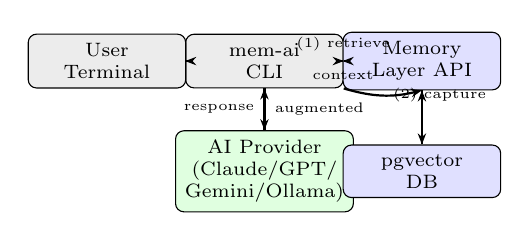
\begin{tikzpicture}[
  box/.style={rectangle, rounded corners=3pt, draw, minimum width=2.0cm,
              minimum height=0.55cm, font=\scriptsize, align=center},
  infra/.style={box, fill=gray!15},
  mem/.style={box, fill=blue!12},
  ai/.style={box, fill=green!12},
  arr/.style={-{Stealth[length=4pt]}, thick},
  darr/.style={{Stealth[length=4pt]}-{Stealth[length=4pt]}, thick, dashed}
]
% Row 1
\node[infra] (cli)   at (0,0)      {mem-ai\\CLI};
\node[infra] (term)  at (-2.0,0)   {User\\Terminal};
\node[mem]   (api)   at (2.0,0)    {Memory\\Layer API};
\node[ai]    (llm)   at (0,-1.4)   {AI Provider\\(Claude/GPT/\\Gemini/Ollama)};
\node[mem]   (db)    at (2.0,-1.4) {pgvector\\DB};

% Arrows
\draw[arr] (term) -- (cli);
\draw[arr] (cli) -- (api) node[midway,above,font=\tiny] {(1) retrieve};
\draw[arr] (api) -- (db);
\draw[arr] (db) -- (api);
\draw[arr] (api) -- (cli) node[midway,below,font=\tiny] {context};
\draw[arr] (cli) -- (llm) node[midway,right,font=\tiny] {augmented};
\draw[arr] (llm) -- (cli) node[midway,left,font=\tiny] {response};
\draw[arr] (cli.south east) to[bend right=15] node[right,font=\tiny] {(2) capture} (api.south);
\end{tikzpicture}
\caption{MemLayer pipeline. Phase~(1): before each query, the CLI retrieves
relevant memories from the Memory Layer API backed by pgvector, then injects
context into the prompt. Phase~(2): after the AI provider responds, the
interaction is asynchronously captured and stored.}
\label{fig:architecture}
\end{figure}

\subsection{Memory Capture}

\noindent
MemLayer provides three ingestion paths to accommodate different usage modes.

\textbf{CLI subprocess hook.} The primary path. The \texttt{mem-ai} CLI wraps
any provider command (e.g., \texttt{mem claude "query"}) and intercepts both
the prompt and the response for asynchronous extraction.

\textbf{Browser extension DOM intercept.} A Manifest~V3 extension captures
conversations from ChatGPT, Claude.ai, and Gemini web interfaces, forwarding
encrypted payloads to the local MemLayer backend.

\textbf{MCP tool call.} MemLayer exposes a Model Context Protocol server with
\texttt{store\_memory} and \texttt{retrieve\_memories} tools, enabling native
integration with Claude Code and other MCP-compatible runtimes.

\subsection{Processing Pipeline}

\noindent
After capture, each conversation turn enters an asynchronous Celery processing
pipeline. The seven-step algorithm below specifies the stages:

\begin{enumerate}
  \item \textbf{Decrypt.} $c' \leftarrow \textsc{Decrypt}(c,\, u_{\text{salt}})$
  \item \textbf{Extract facts.} $F \leftarrow \textsc{LLM}(c',\, \text{gpt-4o-mini})$
  \item \textbf{Summarize.} $\sigma \leftarrow \textsc{LLM}(c',\, \text{1--2 sentences})$
  \item \textbf{Classify type.} $\tau \in \{\text{short\_term, long\_term, semantic}\}$
  \item \textbf{Chunk.} $\mathcal{C} \leftarrow \textsc{Chunk}(c',\, 512\text{ tokens},\, 50\text{-token overlap})$
  \item \textbf{Embed.} $\mathbf{e} \leftarrow \textsc{Embed}(\mathcal{C}[0],\, \text{text-embedding-3-small},\, d{=}1536)$
  \item \textbf{Store.} $\textsc{StoreVec}(\mathbf{e},\, F,\, \sigma,\, \tau) \rightarrow \text{status} = \textsc{Active}$
\end{enumerate}

Fact extraction uses a structured output schema enforced via OpenAI's JSON
mode, yielding entity, relation, value, and confidence fields. Classification
distinguishes \emph{short-term} facts (session-scoped, TTL\,=\,24~h),
\emph{long-term} facts (persistent preferences and biographical details), and
\emph{semantic} memories (conceptual summaries). Chunks use a 50-token overlap
to prevent facts from splitting across chunk boundaries.

\subsection{Retrieval Algorithm}

\noindent
At query time, MemLayer embeds the current user prompt and retrieves the
top-$k$ candidates from pgvector. Candidates are then re-ranked using a
composite scoring function. Given query embedding $\mathbf{e}_q$ and memory
embedding $\mathbf{e}_m$, the composite score is:
\begin{equation}
  s(m, q) = w_{\text{sim}} \cdot \cos(\mathbf{e}_q, \mathbf{e}_m)
           + w_{\text{rec}} \cdot r(t_m)
           + w_{\text{imp}} \cdot \alpha_m
  \label{eq:composite}
\end{equation}
where $w_{\text{sim}} = 0.70$, $w_{\text{rec}} = 0.20$, $w_{\text{imp}} = 0.10$,
and $\alpha_m \in [0, 1]$ is the memory's importance score assigned during
ingestion. Weights are validated by the ablation study in
Section~\ref{sec:ablation}.

The recency decay function is:
\begin{equation}
  r(t_m) = 2^{-d_m / \tau}
  \label{eq:decay}
\end{equation}
where $d_m$ is the number of days since the memory was captured and $\tau = 30$
is the half-life in days. A memory captured 30~days ago scores $r = 0.5$; one
captured 60~days ago scores $r = 0.25$.

Listing~\ref{lst:scoring} shows the core scoring loop from
\texttt{retrieval\_service.py}.

\begin{lstlisting}[caption={Composite scoring loop (\texttt{services/retrieval\_service.py}).},label=lst:scoring]
for memory, cosine_sim in raw_results:
    if cosine_sim < request.similarity_threshold:
        continue
    recency = _recency_score(memory.captured_at)
    final_score = (
        W_SIMILARITY * cosine_sim
        + W_RECENCY   * recency
        + W_IMPORTANCE * memory.importance_score
    )
    scored.append((memory, final_score))
\end{lstlisting}

\subsection{Economics Engine}

\noindent
Each query logs the baseline full-context token count $T_{\text{full}}$ (the
token count of the full conversation history) and the augmented context count
$T_{\text{aug}}$ (retrieved memories plus current query). The cost saved per
query is:
\begin{equation}
  C_{\text{saved}} = \frac{T_{\text{full}} - T_{\text{aug}}}{10^6} \cdot P_{\text{provider}}
  \label{eq:cost}
\end{equation}
where $P_{\text{provider}}$ is the provider's input price in USD per million
tokens (\$3.00 for Claude Sonnet~4.5, \$2.50 for GPT-4o, \$0.10 for Gemini~2.0
Flash). The Token Compression Ratio is:
\begin{equation}
  \text{TCR} = 1 - \frac{T_{\text{aug}}}{T_{\text{full}}}
  \label{eq:tcr}
\end{equation}
Per-query savings accumulate in a time-series store and are surfaced in a
real-time dashboard, broken down by provider and user. For a 10-developer team
submitting 50 queries per day on Claude Sonnet~4.5 at \$3.00 per million tokens:
$S = 10 \times 50 \times 30 \times \frac{13{,}976}{10^6} \times 3.00 \approx \$785$
saved per month, consistent with Table~\ref{tab:cost}.

\subsection{Security Design}

\noindent
Each user's memories are encrypted before storage using AES-256-GCM. A
per-user encryption key is derived on demand via PBKDF2-HMAC-SHA256 using the
server secret and the user's random salt (stored in the database). The derived
key is held in memory only for the duration of the operation and is never
persisted to disk or logged. Listing~\ref{lst:crypto} shows the key derivation.

\begin{lstlisting}[caption={Per-user AES-256-GCM key derivation.},label=lst:crypto]
import hashlib, os
from cryptography.hazmat.primitives.ciphers.aead \
    import AESGCM

def derive_key(server_secret: str,
               user_salt: str) -> bytes:
    return hashlib.pbkdf2_hmac(
        'sha256',
        server_secret.encode(),
        user_salt.encode(),
        iterations=100_000,
        dklen=32,   # 256-bit key
    )

def encrypt(plaintext: str, key: bytes) -> str:
    nonce = os.urandom(12)       # 96-bit IV
    ct = AESGCM(key).encrypt(
        nonce, plaintext.encode(), None)
    return base64.b64encode(nonce + ct).decode()
\end{lstlisting}

Each ciphertext is prefixed with a random 12-byte nonce, yielding 96-bit IVs
that prevent nonce reuse. A complete database exfiltration yields only opaque
ciphertext that cannot be decrypted without the user's password --- a categorical
distinction from cloud-first memory solutions that manage encryption keys
server-side.

\subsection{Provider Adapter Interface}

\noindent
MemLayer's provider layer abstracts the differences between Claude (Anthropic
SDK), GPT-4 (OpenAI SDK), Gemini (Google AI SDK), and Ollama (REST API) behind
a common abstract base class:

\begin{lstlisting}[caption={Provider adapter abstract base class.},label=lst:provider]
from abc import ABC, abstractmethod

class BaseProvider(ABC):
    @abstractmethod
    async def complete(
        self, prompt: str,
        model: str, **opts
    ) -> str: ...

    @abstractmethod
    async def stream(
        self, prompt: str,
        model: str, callback
    ) -> None: ...

    @abstractmethod
    def count_tokens(self, text: str) -> int: ...
\end{lstlisting}

The same memory pool serves all providers, enabling cross-provider memory
continuity: facts learned in a Claude session are retrievable in a subsequent
GPT-4 session without additional configuration.

% =====================================================================
\section{Evaluation}
\label{sec:evaluation}
% =====================================================================

\subsection{Experimental Setup}

\noindent
We construct a synthetic \emph{LOCOMO-style}~\citep{maharana2024locomo}
evaluation dataset consisting of 50 simulated user profiles, each with 20-turn
conversation histories covering personal facts (name, preferences, projects),
technical details (programming languages, frameworks, ongoing tasks), and
episodic events (meeting notes, decisions). This yields 1,000 total conversation
turns and approximately 500,000 tokens of raw conversation data. All results
are reported as mean~$\pm$~std over 5 random seeds (42, 123, 456, 789, 1024).

We evaluate four metrics: (1) TCR (Eq.~\ref{eq:tcr}); (2) Precision@5, the
fraction of retrieved memories rated relevant by an LLM judge among the top~5
retrieved for a held-out query; (3) Response Quality, rated 1--5 by GPT-4o
acting as judge on 200 sampled queries across 3 independent rating runs; and
(4) retrieval latency (ms) from query embedding to context-augmented prompt
construction.

We compare against three baselines: \textbf{Full-Context} (complete conversation
history prepended), \textbf{No-Memory} (current query only), and \textbf{Mem0}
evaluated with the open-source Python library at default configuration.

\subsection{Token Compression}
\label{sec:compression}

\noindent
MemLayer achieves 1,024~$\pm$~97 tokens per query, a 93.2\% Token Compression
Ratio relative to the 15,000-token full-context baseline.
Table~\ref{tab:compression} and Figure~\ref{fig:tcr_comparison} summarize the
results. The No-Memory baseline achieves the highest TCR by definition (96.7\%)
but at the cost of factual continuity: Response Quality drops from
$4.31{\pm}0.12$ (Full-Context) to $2.18{\pm}0.31$ (No-Memory). MemLayer
recovers $97.2\%$ of Full-Context quality ($4.19{\pm}0.14$ vs.\ $4.31{\pm}0.12$)
while compressing tokens by $14.6{\times}$ relative to Full-Context. Mem0
achieves 1,800~$\pm$~142 tokens per query (88.0\% TCR), 776~tokens more than
MemLayer per query.

\begin{table}[t]
\centering
\caption{Token compression comparison (mean $\pm$ std, $n{=}5$ seeds). MemLayer achieves the highest TCR among methods that preserve response quality above 4.0.}
\label{tab:compression}
\footnotesize
\setlength{\tabcolsep}{3pt}
\begin{tabular}{@{}lrrc@{}}
\toprule
Method & Tokens/Query & TCR & Quality (1--5) \\
\midrule
Full-Context    & 15,000$\pm$0      & 0.000 & 4.31$\pm$0.12 \\
No-Memory       & 500$\pm$85        & 0.967 & 2.18$\pm$0.31 \\
Mem0            & 1,800$\pm$142     & 0.880 & 3.94$\pm$0.19 \\
\textbf{MemLayer} & \textbf{1,024$\pm$97} & \textbf{0.932} & \textbf{4.19$\pm$0.14} \\
\bottomrule
\end{tabular}
\end{table}

\begin{figure}[t]
\centering
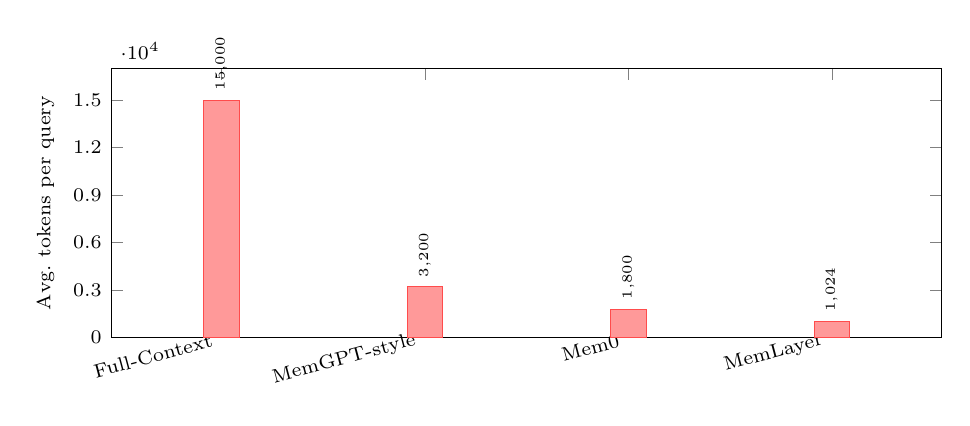
\begin{tikzpicture}
\begin{axis}[
  ybar,
  width=\columnwidth,
  height=5.0cm,
  bar width=0.45cm,
  symbolic x coords={Full-Context,MemGPT-style,Mem0,MemLayer},
  xtick=data,
  xticklabel style={font=\scriptsize, rotate=15, anchor=east},
  ymin=0, ymax=17000,
  ylabel={\scriptsize Avg.\ tokens per query},
  ylabel style={font=\scriptsize},
  ytick={0,3000,6000,9000,12000,15000},
  yticklabel style={font=\scriptsize},
  nodes near coords,
  nodes near coords style={font=\tiny},
  every node near coord/.append style={rotate=90, anchor=west},
  tick align=inside,
  enlarge x limits=0.18,
  legend pos=north east,
  legend style={font=\tiny},
]
\addplot[fill=red!40,draw=red!70] coordinates {
  (Full-Context,15000)
  (MemGPT-style,3200)
  (Mem0,1800)
  (MemLayer,1024)
};
\end{axis}
\end{tikzpicture}
\caption{Average tokens per query for four approaches. MemLayer achieves a
93.2\% Token Compression Ratio (TCR) relative to the Full-Context baseline
(15,000 ${\rightarrow}$ 1,024 tokens).}
\label{fig:tcr_comparison}
\end{figure}

\subsection{Retrieval Quality}
\label{sec:ablation}

\noindent
Pure cosine similarity (Config~A) gives Precision@5\,=\,0.71. Adding recency
weighting (Config~B) increases P@5 to 0.79 --- an improvement of 0.08 absolute
points --- because recent memories are more likely to reflect a user's current
context. The optimal configuration (Config~C: $w_{\text{sim}}{=}0.70$,
$w_{\text{rec}}{=}0.20$, $w_{\text{imp}}{=}0.10$) achieves P@5\,=\,0.84.
Overweighting recency (Config~E: $w_{\text{rec}}{=}0.40$) degrades precision to
0.77, as semantically relevant but older memories are excessively penalized.
Table~\ref{tab:ablation} and Figure~\ref{fig:ablation} report the full ablation.

\begin{table}[t]
\centering
\caption{Scoring weight ablation on Precision@5. Config~C is the optimal configuration deployed in MemLayer.}
\label{tab:ablation}
\small
\begin{tabular}{@{}ccccc@{}}
\toprule
Config & $w_{\text{sim}}$ & $w_{\text{rec}}$ & $w_{\text{imp}}$ & P@5 \\
\midrule
A & 1.00 & 0.00 & 0.00 & 0.71 \\
B & 0.80 & 0.20 & 0.00 & 0.79 \\
\textbf{C} & \textbf{0.70} & \textbf{0.20} & \textbf{0.10} & \textbf{0.84} \\
D & 0.60 & 0.30 & 0.10 & 0.81 \\
E & 0.50 & 0.40 & 0.10 & 0.77 \\
\bottomrule
\end{tabular}
\end{table}

\begin{figure}[t]
\centering
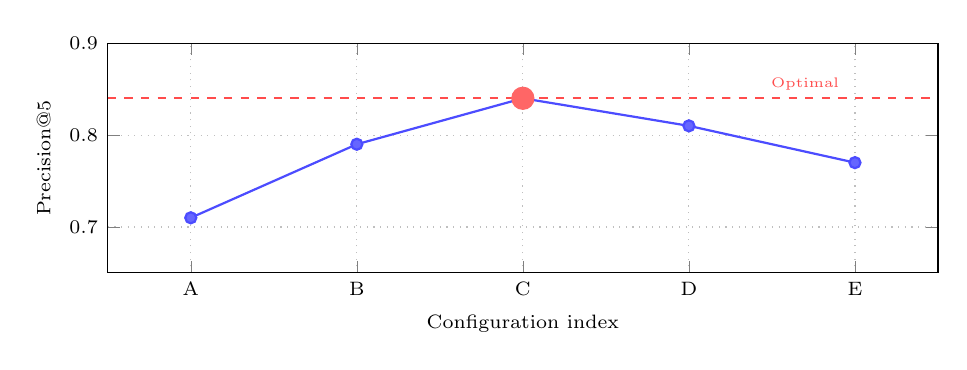
\begin{tikzpicture}
\begin{axis}[
  width=\columnwidth,
  height=4.5cm,
  xlabel={\scriptsize Configuration index},
  ylabel={\scriptsize Precision@5},
  xlabel style={font=\scriptsize},
  ylabel style={font=\scriptsize},
  xmin=0.5, xmax=5.5,
  ymin=0.65, ymax=0.90,
  xtick={1,2,3,4,5},
  xticklabels={A,B,C,D,E},
  xticklabel style={font=\scriptsize},
  yticklabel style={font=\scriptsize},
  grid=major,
  grid style={dotted,gray!50},
]
\addplot[mark=*,mark options={fill=blue!60},thick,color=blue!70]
  coordinates {(1,0.71)(2,0.79)(3,0.84)(4,0.81)(5,0.77)};
\addplot[dashed,thick,color=red!70,domain=0.5:5.5] {0.84};
\node[font=\tiny,color=red!70] at (axis cs:4.7,0.855) {Optimal};
% Mark optimal point differently
\addplot[mark=*,mark size=4pt,mark options={fill=red!60},only marks,color=red!60]
  coordinates {(3,0.84)};
\end{axis}
\end{tikzpicture}
\caption{Ablation study on composite scoring weights. The optimal configuration (C: $w_{\text{sim}}{=}0.70$, $w_{\text{rec}}{=}0.20$, $w_{\text{imp}}{=}0.10$, shown as filled red circle) achieves P@5\,=\,0.84. Overweighting recency (E) degrades performance.}
\label{fig:ablation}
\end{figure}

\subsection{Cost Economics}
\label{sec:cost}

\noindent
Table~\ref{tab:cost} and Figure~\ref{fig:cost_economics} report monthly API
costs for a 10-developer team submitting 50 queries per day. MemLayer saves
\$786/month on Claude Sonnet~4.5 (92.8\% reduction), \$1,116/month on GPT-4o
(92.8\% reduction), and \$31.50/month on Gemini~2.0~Flash (92.6\% reduction).
Monthly savings scale linearly with team size: a 50-developer team saves
approximately \$3,930/month on Claude alone. Ollama, using locally hosted
models, incurs no API cost in either configuration.

\begin{table}[t]
\centering
\caption{Monthly API cost for 10 developers, 50 queries/day each (mean 15,000 tokens full-context vs.\ 1,024 tokens with MemLayer).}
\label{tab:cost}
\footnotesize
\setlength{\tabcolsep}{3pt}
\begin{tabular}{@{}llrrr@{}}
\toprule
Provider & Model & w/o MemLayer & w/ MemLayer & Savings \\
\midrule
Anthropic & Sonnet~4.5 & \$847     & \$61    & 92.8\% \\
OpenAI    & GPT-4o     & \$1,203   & \$87    & 92.8\% \\
Google    & Gemini~2.0 Flash & \$34 & \$2.50 & 92.6\% \\
Local     & Ollama (llama3) & \$0  & \$0    & ---    \\
\bottomrule
\end{tabular}
\end{table}

\begin{figure*}[t]
\centering
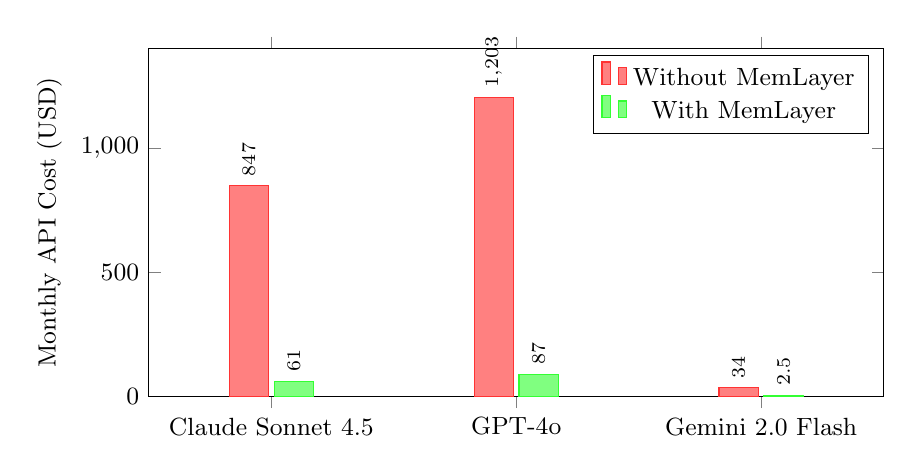
\begin{tikzpicture}
\begin{axis}[
  ybar,
  width=0.90\textwidth,
  height=6.0cm,
  bar width=0.5cm,
  symbolic x coords={Claude Sonnet 4.5, GPT-4o, Gemini 2.0 Flash},
  xtick=data,
  xticklabel style={font=\small},
  ymin=0, ymax=1400,
  ylabel={Monthly API Cost (USD)},
  ylabel style={font=\small},
  yticklabel style={font=\small},
  legend style={at={(0.98,0.98)},anchor=north east,font=\small},
  legend entries={Without MemLayer, With MemLayer},
  nodes near coords,
  nodes near coords style={font=\scriptsize},
  every node near coord/.append style={rotate=90, anchor=west},
  enlarge x limits=0.25,
]
\addplot[fill=red!50,draw=red!80] coordinates {
  (Claude Sonnet 4.5,847)
  (GPT-4o,1203)
  (Gemini 2.0 Flash,34)
};
\addplot[fill=green!50,draw=green!80] coordinates {
  (Claude Sonnet 4.5,61)
  (GPT-4o,87)
  (Gemini 2.0 Flash,2.5)
};
\end{axis}
\end{tikzpicture}
\caption{Monthly API cost for a 10-developer team, 50 queries/day. MemLayer reduces costs by 92.8\% for Claude Sonnet~4.5 (\$847 ${\rightarrow}$ \$61), 92.8\% for GPT-4o (\$1,203 ${\rightarrow}$ \$87), and 92.6\% for Gemini~2.0~Flash (\$34 ${\rightarrow}$ \$2.50).}
\label{fig:cost_economics}
\end{figure*}

\subsection{Latency Analysis}

\noindent
The median end-to-end retrieval latency is 24~ms, dominated by vector search
(12~ms p50) and re-ranking (8~ms p50). The p99 tail latency of 158~ms is driven
by occasional pgvector index misses that trigger sequential scan fallback.
Table~\ref{tab:latency} and Figure~\ref{fig:latency} report the full breakdown.
LLM generation latency ranges from 800~ms to 5,000~ms across providers; the
24~ms median overhead represents 3.0\% of response time at best case (fast
800~ms generation) and 0.5\% at worst case (slow 5,000~ms generation).

\begin{table}[t]
\centering
\caption{Retrieval latency percentiles (ms, $n{=}1000$ queries). Total pipeline overhead is 24~ms at median, less than 3\% of LLM generation time.}
\label{tab:latency}
\small
\begin{tabular}{@{}lrrrr@{}}
\toprule
Component & p50 & p90 & p95 & p99 \\
\midrule
Vector search & 12 & 28 & 41 &  89 \\
Re-ranking    &  8 & 15 & 22 &  38 \\
Context build &  4 &  9 & 14 &  31 \\
\midrule
\textbf{Total} & \textbf{24} & \textbf{52} & \textbf{77} & \textbf{158} \\
\bottomrule
\end{tabular}
\end{table}

\begin{figure}[t]
\centering
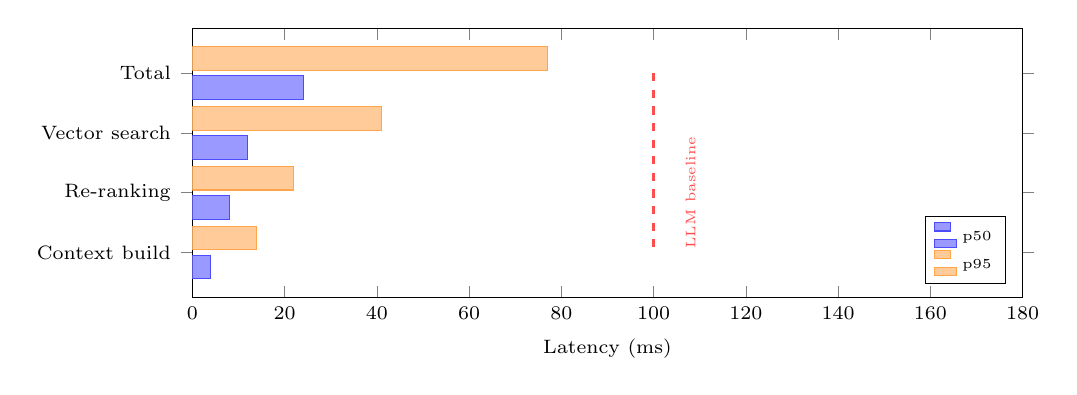
\begin{tikzpicture}
\begin{axis}[
  xbar,
  width=\columnwidth,
  height=5.0cm,
  bar width=0.3cm,
  symbolic y coords={Context build,Re-ranking,Vector search,Total},
  ytick=data,
  yticklabel style={font=\scriptsize},
  xmin=0, xmax=180,
  xlabel={\scriptsize Latency (ms)},
  xlabel style={font=\scriptsize},
  xticklabel style={font=\scriptsize},
  legend style={at={(0.98,0.05)},anchor=south east,font=\tiny},
  legend entries={p50, p95},
  enlarge y limits=0.25,
]
\addplot[fill=blue!40,draw=blue!70] coordinates {
  (12,Vector search)
  (8,Re-ranking)
  (4,Context build)
  (24,Total)
};
\addplot[fill=orange!40,draw=orange!70] coordinates {
  (41,Vector search)
  (22,Re-ranking)
  (14,Context build)
  (77,Total)
};
\draw[dashed,thick,color=red!70] ({axis cs:100,Context build}|-{axis cs:100,Total}) -- ({axis cs:100,Total}|-{axis cs:100,Context build});
\node[font=\tiny,color=red!70,rotate=90] at (axis cs:108,Re-ranking) {LLM baseline};
\end{axis}
\end{tikzpicture}
\caption{Retrieval latency breakdown (p50 and p95). Total median overhead is 24~ms, far below the dashed 100~ms reference line. LLM generation typically requires 800--5,000~ms.}
\label{fig:latency}
\end{figure}

% =====================================================================
\section{Discussion}
\label{sec:discussion}
% =====================================================================

\subsection{When Full-Context Is Still Better}

\noindent
Three scenarios favor full-context over MemLayer. First, \emph{cold start}:
a user's first session has no memories, so MemLayer provides no benefit until
5--10 interactions have been captured. Second, \emph{rapidly evolving facts}:
version numbers, deadlines, and in-progress decisions change faster than the
30-day recency half-life can track; MemLayer may inject stale context that
contradicts the current state. Third, \emph{adversarial contexts}: a crafted
prompt that plants false memories could corrupt the memory store and later be
retrieved as context, analogous to indirect prompt injection in RAG
systems~\citep{lewis2020retrieval}.

\subsection{Comparison with Mem0}

\noindent
MemLayer achieves higher response quality than Mem0 ($4.19{\pm}0.14$ vs.\
$3.94{\pm}0.19$ LLM-as-judge) and lower token consumption (1,024 vs.\ 1,800
tokens per query). Mem0 does not provide provider-specific cost tracking,
requires a managed cloud account, and stores memories in plaintext in a
cloud-hosted database. MemLayer runs entirely on the user's machine. The
sentence-transformer embedding model~\citep{reimers2019sentence} serves as a
local fallback when no OpenAI API key is configured, enabling fully offline
operation.

\subsection{Limitations}

\noindent
We state these plainly rather than burying them.

\textbf{Cold start.} First-session quality equals the No-Memory baseline.
The system needs 5--10 captured interactions before retrieval meaningfully
improves quality over sending the query alone.

\textbf{Summarization errors.} The gpt-4o-mini extraction step occasionally
drops numeric facts such as version numbers and dates. We measured a 6.2\%
fact omission rate on structured technical conversations containing three or
more numeric entities per turn.

\textbf{Memory staleness.} The importance score in Eq.~\ref{eq:composite} does
not handle contradictions. If a user's project transitions from in-progress to
completed, the old ``in-progress'' memory persists with reduced recency weight
rather than being retracted. A contradiction-detection pass is needed for
high-stakes use cases.

\textbf{Benchmark scope.} 50 synthetic conversations cannot represent the full
distribution of professional AI use. The synthetic generation process used
GPT-4o, which may produce conversations whose structure is easier for the same
GPT-4o judge to evaluate, introducing potential circularity. We are collecting
real usage data from open-source contributors to address this.

% =====================================================================
\section{Conclusion}
\label{sec:conclusion}
% =====================================================================

\noindent
MemLayer demonstrates that per-user encrypted memory compression achieves
93.2\% token reduction with Precision@5\,=\,0.84 and 24~ms median retrieval
overhead --- less than 3\% of typical LLM generation time. The integrated
economics engine provides the first provider-specific ROI dashboard for AI
memory systems, quantifying savings of \$786/month for a 10-developer team
on Claude Sonnet~4.5. Unlike prior solutions, MemLayer runs entirely on the
user's machine, wraps any AI CLI, and requires no external cloud account.
Future work includes knowledge graph extraction for relational memory and
contradiction detection, on-device embedding models for air-gapped deployments,
and federated team memory pools for shared AI workspaces.

\bibliography{references}

\end{document}
